\clearpage

\section{Modifying and applying Grad-CAM}
\nblink{brats/07\_gradcam.ipynb}

The basic idea how to apply interpretability methods built for classification on image segmentation tasks is quite simple: The output of a classification model
is a list of confidence scores, one for every class the model can detect. In a segmentation task, the output is a list of pixels with an intensity value.
What we can do is interpret every output pixel as if was a separate class in a classification task.
In a classification task, we are only interested in the highest class value. In a segmentation task, we are interested why a specific pixel from the ground truth did
or did not show up in the network output.

As a first step, we can analyze a saliency map generated for a single class. In the following Result chapter, we analyze the pixel indicated by a red dot.

\clearpage

\subsection{Results}

Figure \ref{grad_cam_brats_result} shows the Grad-CAM output of multiple layers of the neural network. Grad-CAM for classification is applied on the last convolutional layer
of the network, but in this case this produced no output at all (Image (i) in the figure). We therefore decided to also analyze other layers (batch normalization and convolutional layers)
to see if there is any insight how the network came up with the output segmentation.

\begin{figure}[H]\ContinuedFloat
    \centering
    \begin{subfigure}{.32\textwidth}
        \centering
        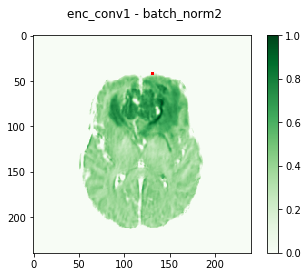
\includegraphics[width=\linewidth]{chapters/04_segmentation/images/grad_cam_03.png}
        \caption{First batch norm layer of the first encoder block}
    \end{subfigure}\hfill%
    \begin{subfigure}{.32\textwidth}
        \centering
        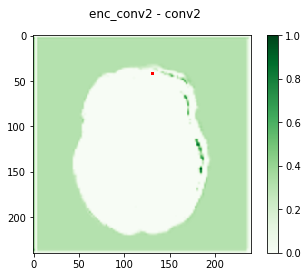
\includegraphics[width=\linewidth]{chapters/04_segmentation/images/grad_cam_05.png}
        \caption{Second convolutional layer in the second encoder block}
    \end{subfigure}\hfill%
    \begin{subfigure}{.32\textwidth}
        \centering
        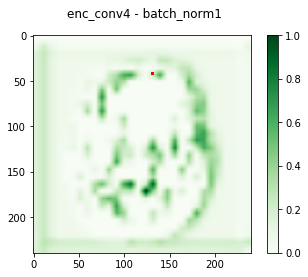
\includegraphics[width=\linewidth]{chapters/04_segmentation/images/grad_cam_14.png}
        \caption{First batch norm layer of the 4. encoder block}
    \end{subfigure}

    \begin{subfigure}{.33\textwidth}
        \centering
        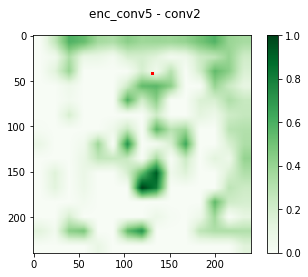
\includegraphics[width=\linewidth]{chapters/04_segmentation/images/grad_cam_17.png}
        \caption{Second convolutional layer of the 5. encoder block}
    \end{subfigure}\hfill%
    \begin{subfigure}{.32\textwidth}
        \centering
        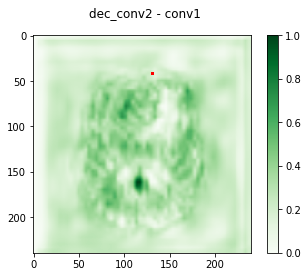
\includegraphics[width=\linewidth]{chapters/04_segmentation/images/grad_cam_24.png}
        \caption{First convolutional layer of the second decoder block}
    \end{subfigure}\hfill%
    \begin{subfigure}{.32\textwidth}
        \centering
        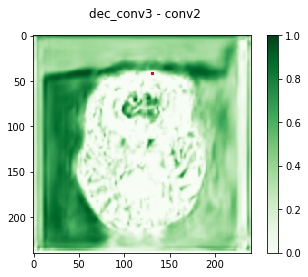
\includegraphics[width=\linewidth]{chapters/04_segmentation/images/grad_cam_29.png}
        \caption{Second convolutional layer of the third decoder block}
    \end{subfigure}

    \begin{subfigure}{.33\textwidth}
        \centering
        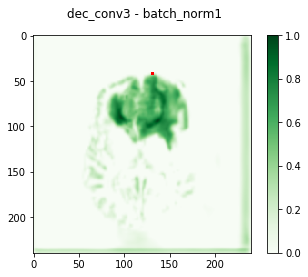
\includegraphics[width=\linewidth]{chapters/04_segmentation/images/grad_cam_30.png}
        \caption{First batch norm layer of the third decoder block}
    \end{subfigure}\hfill%
    \begin{subfigure}{.32\textwidth}
        \centering
        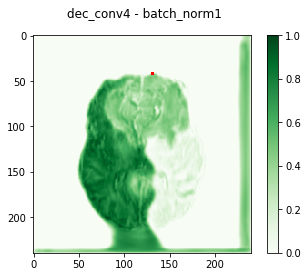
\includegraphics[width=\linewidth]{chapters/04_segmentation/images/grad_cam_34.png}
        \caption{First batch norm layer of the 4. decoder block}
    \end{subfigure}\hfill%
    \begin{subfigure}{.32\textwidth}
        \centering
        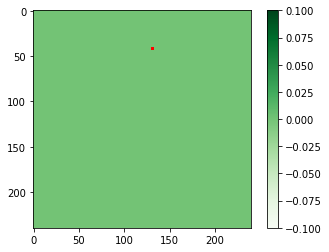
\includegraphics[width=\linewidth]{chapters/04_segmentation/images/grad_cam_36.png}
        \caption{Output convolutional layer}
    \end{subfigure}
    \caption{Grad-CAM output of the first pixel of the ground truth output segment (red pixel). No layers provided any significant insight into how the network came to the output segment.}
    \label{grad_cam_brats_result}
\end{figure}

\clearpage

\subsection{Discussion}
\nblink{brats/25\_flair\_threshold.ipynb}
None of the generated outputs provide good insight into the inner workings of the network. The output of the batch normalization layer of the third decoder (Image (g) in Figure \ref{grad_cam_brats_result}) shows the most promising output. But this output can easily be replicated by taking the FLAIR modality and applying a threshold, as seen in Figure \ref{grad_cam_treshold}.

\begin{figure}[H]
\centering
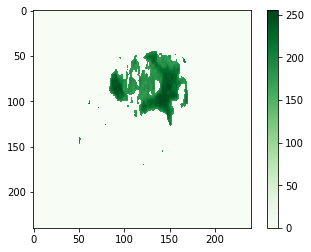
\includegraphics[width=8cm]{chapters/04_segmentation/images/flair_treshold.png}
\captionsetup{width=12cm}
\caption{FLAIR modality with an applied threshold of 170, setting all pixels lower than this value to zero. Shows a very similar shape as image (g) in Figure \ref{grad_cam_brats_result}}
\label{grad_cam_treshold}
\end{figure}


\subsection{Conclusion}
Because of these very underwhelming results, we decided to not modify Grad-CAM to work on multiple pixels and move to other methods.
